	\section{Sensores de temperatura}
	Un sensor de temperatura es un dispositivo que proporciona la medición de temperatura a través de una señal eléctrica. \\
		
	Se utilizan en diversas aplicaciones tales como elaboración de alimentos, climatización para control ambiental, dispositivos médicos, manipulación de productos químicos y control de dispositivos en el sector automotriz, entre otros. \\
		
	Los sensores de temperatura se utilizan para asegurar que la temperatura de algún objeto se encuentre dentro de un cierto rango, lo que proporciona seguridad en el uso de la aplicación. \\
		
	Dependiendo del dispositivo en el que se instalará el sensor de temperatura y el propósito de la aplicación, se deberá utilizar un tipo específico de sensor para medir la temperatura de manera precisa y eficiente, pues en muchos casos la capacidad de respuesta y precisión del circuito de detección puede ser crítica para una pronta decisión.\\
	
	Algunos de los tipos más comunes de sensores de temperatura son los siguientes:
	
	\subsection{Termistores}
	Un termistor es un elemento con una resistencia eléctrica que cambia en respuesta a la temperatura. Este nombre se deriva del término más descriptivo "resistencia térmicamente sensible".\\
						
	Los termistores son un tipo de semiconductor, lo que significa que tienen mayor resistencia que los materiales conductores, pero menor resistencia que los materiales aislantes. La relación entre la temperatura de un termistor y su resistencia depende en gran medida de los materiales de los que está compuesta.\\
			
	Existen dos clases de termistores los que presentan un coeficiente negativo de temperatura (NTC), cuya resistencia disminuye con la temperatura y coeficiente positivo con la temperatura  (PTC) cuya resistencia aumenta con la temperatura. Los termistores NTC son los más usados para medición de temperatura.
			
	\subsection{Circuitos integrados}
	Un sensor de temperatura IC es un transductor de temperatura de circuito integrado de dos terminales que produce una corriente de salida proporcional a la temperatura absoluta. Debido a que son circuitos activos construidos utilizando procesos de semiconductores convencionales, pueden tomar una variedad de formas e incluir una variedad de características (como interfaces digitales y entradas ADC) no disponibles en otras tecnologías. El rango de temperatura de funcionamiento para este tipo de sensores se extiende desde -55 $^{\circ}$C y hasta 125 $^{\circ}$C, con algunos productos operando hasta un límite superior de alrededor de 150 $^{\circ}$C. Dependiendo de la salida que proporcione el sensor, puede clasificarse como analógico o digital:
	
	\subsubsection{Sensor de temperatura analógico}
				Los sensores de temperatura analógicos convierten la temperatura en voltaje o, en algunos casos, en corriente. Los más simples tienen sólo tres conexiones activas: tierra, alimentación y salida. Otros sensores analógicos con características mejoradas pueden tener entradas o salidas adicionales, por ejemplo, salidas de referencia de voltaje o comparador. Estos utilizan las características térmicas de los transistores bipolares para desarrollar un voltaje de salida proporcional a la temperatura.
				
	\subsubsection{Sensor de temperatura digital}
	Se denomina sensor de temperatura digital a un dispositivo que integra un sensor de temperatura analógico con un convertidor analógico-digital (ADC), lo que proporciona una interfaz digital directa.\\
				
    \textbf{Otras características del sensor de temperatura digital}\\
    Además de la función básica de detección de temperatura, los sensores digitales pueden incluir otras características útiles, algunas de las más comunes son:
    \begin{itemize}
    	\item \textbf{Salidas dependiendo de la temperatura:} La mayoría de los sensores de temperatura digitales incluyen una o más salidas que indican que la temperatura medida ha superado un límite preestablecido (generalmente programable por software). La salida puede comportarse como una salida de comparador, con un estado cuando la temperatura está por encima del umbral y el otro estado cuando la temperatura está por debajo del umbral.
    	
    	\item \textbf{Cola de fallos:} Cuando comúnmente ocurren variaciones de temperatura a corto plazo, es posible que prefiera que la salida dependiendo de la temperatura no se afirme como resultado de una única medición de umbral. En su lugar, puede ser mejor afirmar la salida solo después de que hayan tenido lugar algunas mediciones de umbral por encima consecutivas. Una cola de fallas le permite seleccionar el número de mediciones de umbral por encima del umbral requerido antes de que se confirme la salida.
    	
    	\item \textbf{Interfaces:} Los sensores de temperatura digitales están disponibles con una amplia variedad de interfaces digitales que incluyen I2C, SMBus ™, SPI ™, 1-Wire® y PWM.
    \end{itemize}
	
			
	\subsection{Termopares}
	Los termopares se usan comúnmente para medir temperaturas más altas y rangos de temperatura más grandes.\\
			
	Este tipo de sensor de temperatura consta de dos cables de diferentes metales conectados en dos puntos. La tensión variable entre estos dos puntos refleja cambios proporcionales en la temperatura. La precisión es baja, de 0.5 $^{\circ}$C a 5 $^{\circ}$C. Sin embargo, operan en el rango de temperatura más amplio, de -200 $^{\circ}$C a 1750 $^{\circ}$C.			
	
	
	\section{Sensores de pulso}
	
	Para medir el ciclo cardíaco y obtener medidas de la frecuencia cardíaca, existen múltiples técnicas basadas en sensores, sin embargo los dos métodos más utilizados son la electrocardiografía (ECG, también conocida como EKG) y la fotopletismografía (PPG). \\
	
	El sensor de pulso básico de ECG consiste, por lo general, en un bloque de acondicionamiento de señal integrado para ECG, diseñado para extraer, amplificar y filtrar pequeñas señales biopotenciales. Aunque la cantidad de electricidad es, de hecho, muy pequeña, se puede medir de manera confiable con electrodos de ECG adheridos a la piel. El electrodo Ag/AgCl es el más utilizado para todas las aplicaciones de sistemas de electrodos biológicos usados para monitorear y registrar biopotenciales. \\
	
	Por otra parte, el sensor de pulso básico de PPG consiste en un diodo emisor de luz y un detector como una resistencia de detección de luz o un fotodiodo. 

	\subsection{Electrocardiografía}
		La electrocardiografía mide la actividad eléctrica del corazón mediante el uso de electrodos colocados en la piel. Para que el corazón se contraiga y bombee sangre, el sistema nervioso autónomo envía al corazón una serie de señales eléctricas coordinadas. \\
		
		A pesar de que se producen en el interior del cuerpo, estas señales se pueden medir al nivel de la piel utilizando dos o más electrodos colocados en varias posiciones en el pecho y las extremidades. Lo que resulta es un patrón informativo de actividad eléctrica llamado onda de ECG. \\
		
		Aunque hay muchos aspectos de esta señal que pueden cuantificarse, la característica más prominente se conoce como el complejo QRS, que indica las principales contracciones de bombeo del corazón. En la imagen \ref{fig:ECGwave} se muestra la curva de ECG clásica con sus formas de onda más comunes, intervalos importantes y puntos de medición. \\
		
		\begin{figure}[htbp!]
			\centering
			\fbox{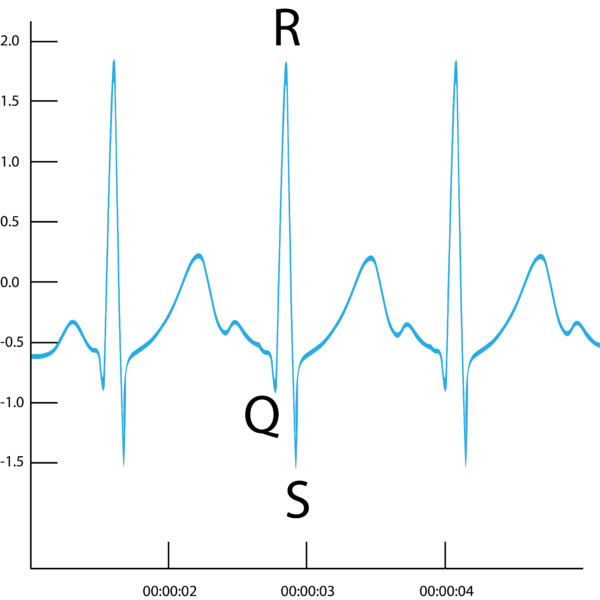
\includegraphics[width=0.6\textwidth]{MarcoTeorico/imagenes/ECGwave.png}}
			\caption{Ondas del ECG.}
			\label{fig:ECGwave}
		\end{figure}
		
		Dentro del complejo QRS, podemos ver el pico R, el componente más prominente dentro de la forma de onda del ECG. Esto es lo que utilizan los algoritmos de frecuencia cardíaca para medir la cantidad de tiempo que ocurre entre cada pulso cardiaco. \\
		
		Debido a que las mediciones basadas en ECG son de señales eléctricas, son generalmente precisas en un par de milisegundos, lo que la convierte en una medida confiable de la frecuencia cardíaca.
		
		\subsection{Fotopletismografía}
			La fotopletismografía mide el cambio volumétrico del corazón midiendo la transmisión de luz o la reflexión. A medida que el corazón se contrae, la presión arterial dentro del ventrículo izquierdo, la cámara de bombeo principal, aumenta. Este aumento obliga a un "pulso" a las arterias del cuerpo, lo que hace que se inflamen ligeramente antes de volver una vez más a su estado anterior. La fotopletismografía puede clasificarse en dos tipos: \\
			
			\begin{itemize}
				\item Transmisión: la luz emitida desde el dispositivo emisor de luz se transmite a través de cualquier región vascular del cuerpo como el lóbulo de la oreja y es recibida por el detector.
				\item Reflexión: la luz emitida desde el dispositivo emisor de luz se refleja en alguna región.
			\end{itemize}
			
			Simplemente al iluminar una región de piel con una fuente de luz LED, el aumento de la presión del pulso causará una diferencia en la cantidad de luz reflejada o transmitida a través de un sensor de luz. La luz LED debe colocarse en un área donde las arterias estén cerca de la piel, como la punta de un dedo o el lóbulo de una oreja. \\
			
			La amplitud de esta señal es directamente proporcional a la presión del pulso: cuanto más alto es el pico, más fuerte es el pulso. Aunque la señal puede ser menos aparente si se mide en la piel en un punto alejado del corazón (como un dedo del pie), el cambio en la presión es suficiente para expandir estas arterias hasta un grado que sea medible. \\
			
			Cada pico en la señal resultante puede identificarse mediante un algoritmo especial de frecuencia cardíaca que puede determinar en última instancia la cantidad de tiempo que ocurre entre cada pico sucesivo, lo que proporciona otra medida de la frecuencia cardíaca. En la imagen \ref{fig:PPGwave} se muestra la curva de PPG con sus formas de onda más comunes y puntos de medición. \\
		
		\begin{figure}[htbp!]
			\centering
			\fbox{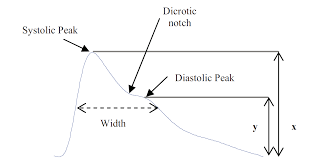
\includegraphics[width=0.7\textwidth]{MarcoTeorico/imagenes/PPGwave.png}}
			\caption{Ondas del PPG.}
			\label{fig:PPGwave}
		\end{figure}
			
			Debido a que la PPG es una técnica que no mide directamente la actividad cardiaca, no siempre es precisa al nivel de milisegundos como las mediciones del ECG, pero es una mancera sencilla para medir la frecuencia cardíaca de una persona ya que utilizan sensores secos y se pueden colocar más rápido en comparación con las configuraciones de ECG, lo que hace que su uso sea más fácil y menos molesto para el usuario.
		
	\section{Microcontroladores}
	Un microcontrolador es  un  circuito  integrado  que  contiene  un  microprocesador  de  forma  interna,  con  todos  los  componentes  para  poder  funcionar  de  forma  autónoma. Aunque los recursos internos del microcontrolador no pueden ser modificados, es posible agregar nuevos recursos de forma externa mediante el uso de interfaces de comunicación como UART, I2C y SPI.\\
	
	Los  elementos  que  generalmente  integran  un  microcontrolador  son:
	\begin{itemize}
		\item Microprocesador.
		\item Memoria  de  datos  RAM.
		\item Memoria  de  programa  ROM/PROM/EPROM.
		\item Módulos  de  E/S  para  comunicarse  con  el  exterior.
		\item Módulos  para  el  control  de  procesos.
		\item Oscilador  interno  para  generar  la  señal  de  reloj.
	\end{itemize}

	